%1. ¿La entropía de la fuente S es máxima? ¿Que sugiere esto acerca de la red? ¿Está relacionado con el
%overhead impuesto por la red debido a los protocolos de control (i.e.: ARP)?
\textbf{Datos obtenidos con la fuente $S$:}

\begin{center}
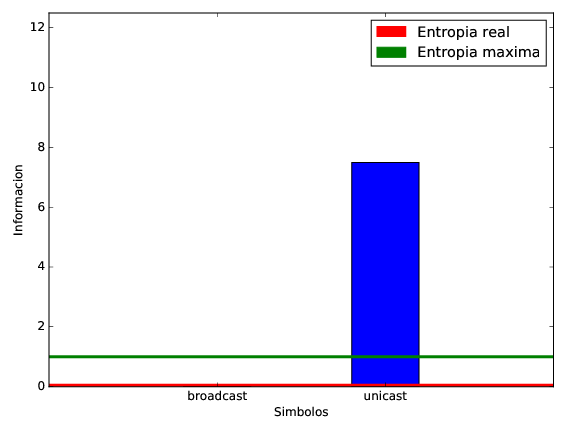
\includegraphics[scale=0.6]{imagenes/analisisTCORPcableada/fuenteS.png} 
\end{center}

Como se puede observar hay muchísimos más broadcast que unicast, es por ello que el último dá más información. Las probabilidades son las siguientes: broadcast 0.99, unicast 0.01. La entropía es 0.049, casi nula.\\

Los broadcast son visibles para todos los dispositivos, mientras que los unicast no. Al ser una red switcheada, nosotros estamos viendo los broadcast de todos los hosts y sólo nuestros unicast (respuestas enviadas al host con el cuál se hizo la captura), es por esto que la diferencia es tan grande.\\

%2. ¿Cómo es el tráfico ARP en la red? ¿Se pueden distinguir nodos? ¿Cuántos? ¿Indica algo la cantidad?
%¿Se les puede adjudicar alguna función específica? ¿Hay evidencia parcial que sugiera que algún nodo
%funciona de forma anómala y/o no esperada?
%3. ¿Existe una correspondencia entre lo que se conoce de la red y los nodos distinguidos detectados por
%la herramienta? ¿Es posible usar el criterio de distinción propuesto como método para descubrir el/los
%Default Gateway/s de la red? ¿Es preciso?
\textbf{Datos obtenidos con la fuente $S1$:}

\begin{center}
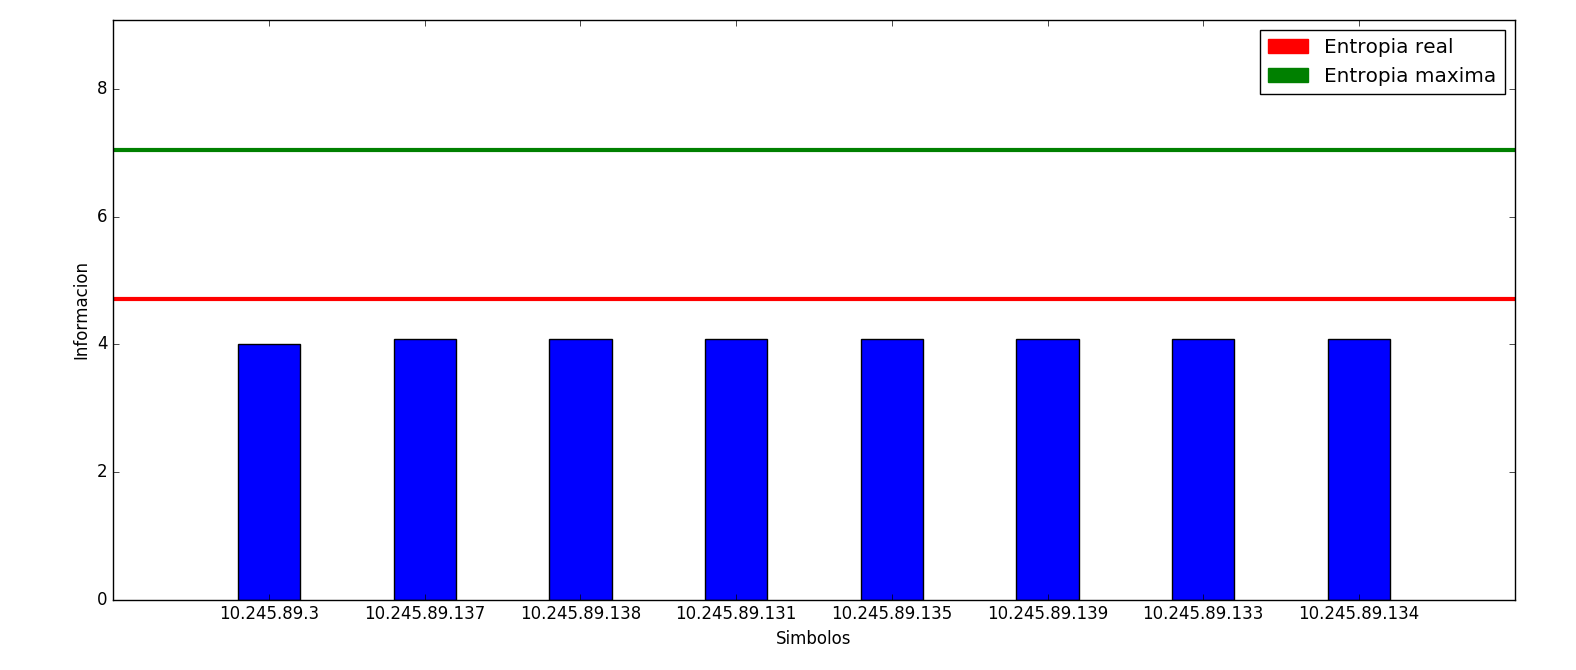
\includegraphics[scale=0.4]{imagenes/analisisTCORPcableada/fuenteS1-11.png} 
\end{center}

Observando la disposición de la red descubrimos manualmente que posee dos IP físicas de gateways, 10.245.89.3 y 10.245.89.2 y una IP que actúa como balanceador, 10.245.89.1, a la cuál los hosts realizan sus pedidos y ésta los redirecciona a 10.245.89.3 o 10.245.89.2 según la carga de cada uno.

\begin{center}
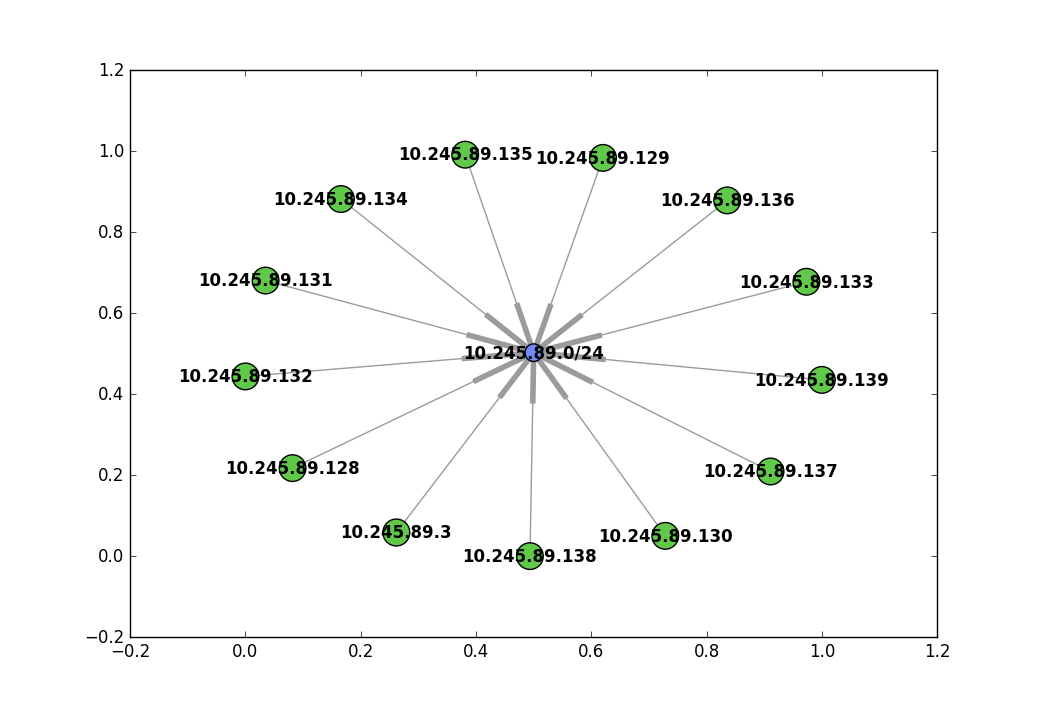
\includegraphics[scale=0.65]{imagenes/analisisTCORPcableada/cableada-11sum.png} 
\end{center}
\vspace*{-1cm}

Los nodos distinguidos que vemos en el gráfico son hosts con mucha actividad, los cuáles están consultando a 10.245.89.1. Quien se encuentra incluído en la red ya que recibe pedidos pero las respuestas a estos son emitidas por 10.245.89.3 o 10.245.89.2 entonces no llega a ser distinguido si nuestros símbolos son los IP de origen.

Dentro de estos nodos distinguidos también se encuentra una de los IP físicas de los gateways, 10.245.89.3. Quién queda ocluído por la actividad de los demás equipos.\\

Como no obtuvimos buenos resultados a la hora de detectar el default gateway, probamos con otra fuente a la cuál llamaremos $S2$, que tiene como símbolos los IP destino de los paquetes ARP Who-Has.\\

Para esta nueva fuente los datos obtenidos son los siguientes:
\begin{center}
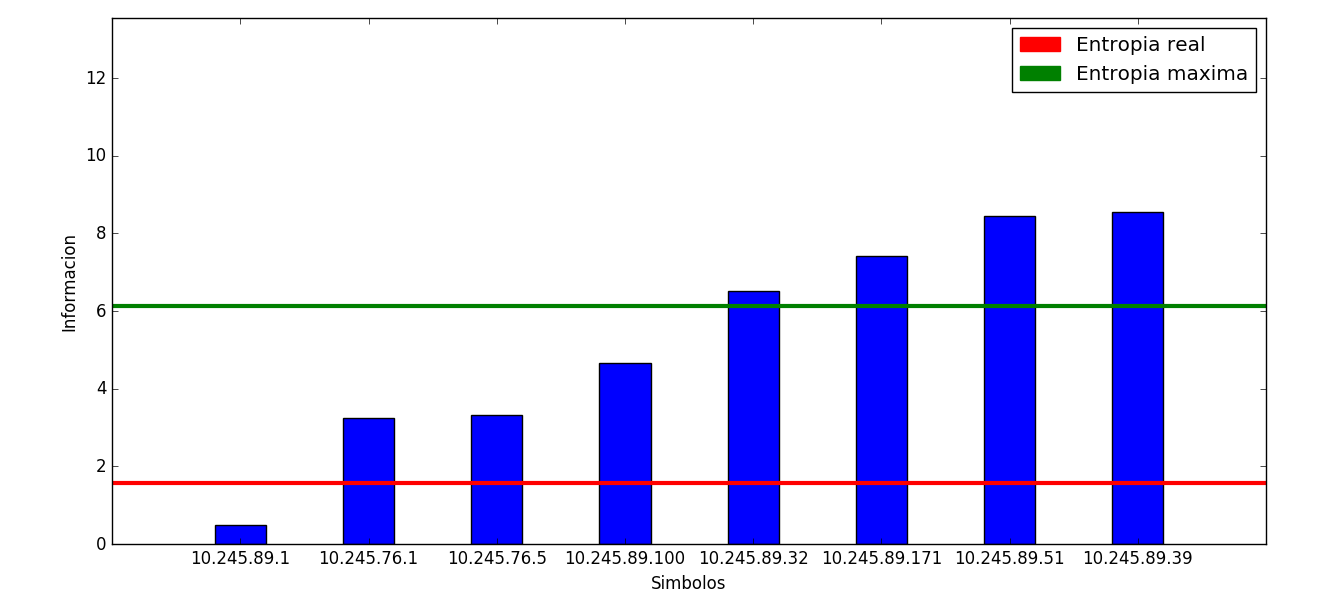
\includegraphics[scale=0.5]{imagenes/analisisTCORPcableada/fuenteS1-12.png} 
\end{center}

En este caso hay un solo nodo distinguido. El cuál, como vimos antes, es el balanceador. Éste es el default gateway para toda la red, quien se encarga de redirigir los pedidos.\\

Todos los equipos en la Lan preguntan la MAC del default gateway para actualizar sus tablas, lo hacen mediante broadcast a nivel de enlace con lo cual el paquete lo ven todos los nodos en dominio de broadcast, en particular la maquina con la que efectuamos la captura.\\

El motivo por el cuál funciona mejor la fuente $S2$ que la $S1$ en este caso, suponemos que se debe tanto al tipo de conexión (ethernet switcheada) como a la disposición (i.e. el hecho de que tenga un balanceador distinto de las IP físicas de los gateways).

\begin{figure}[htbp]
\hspace*{-2cm}                                                           
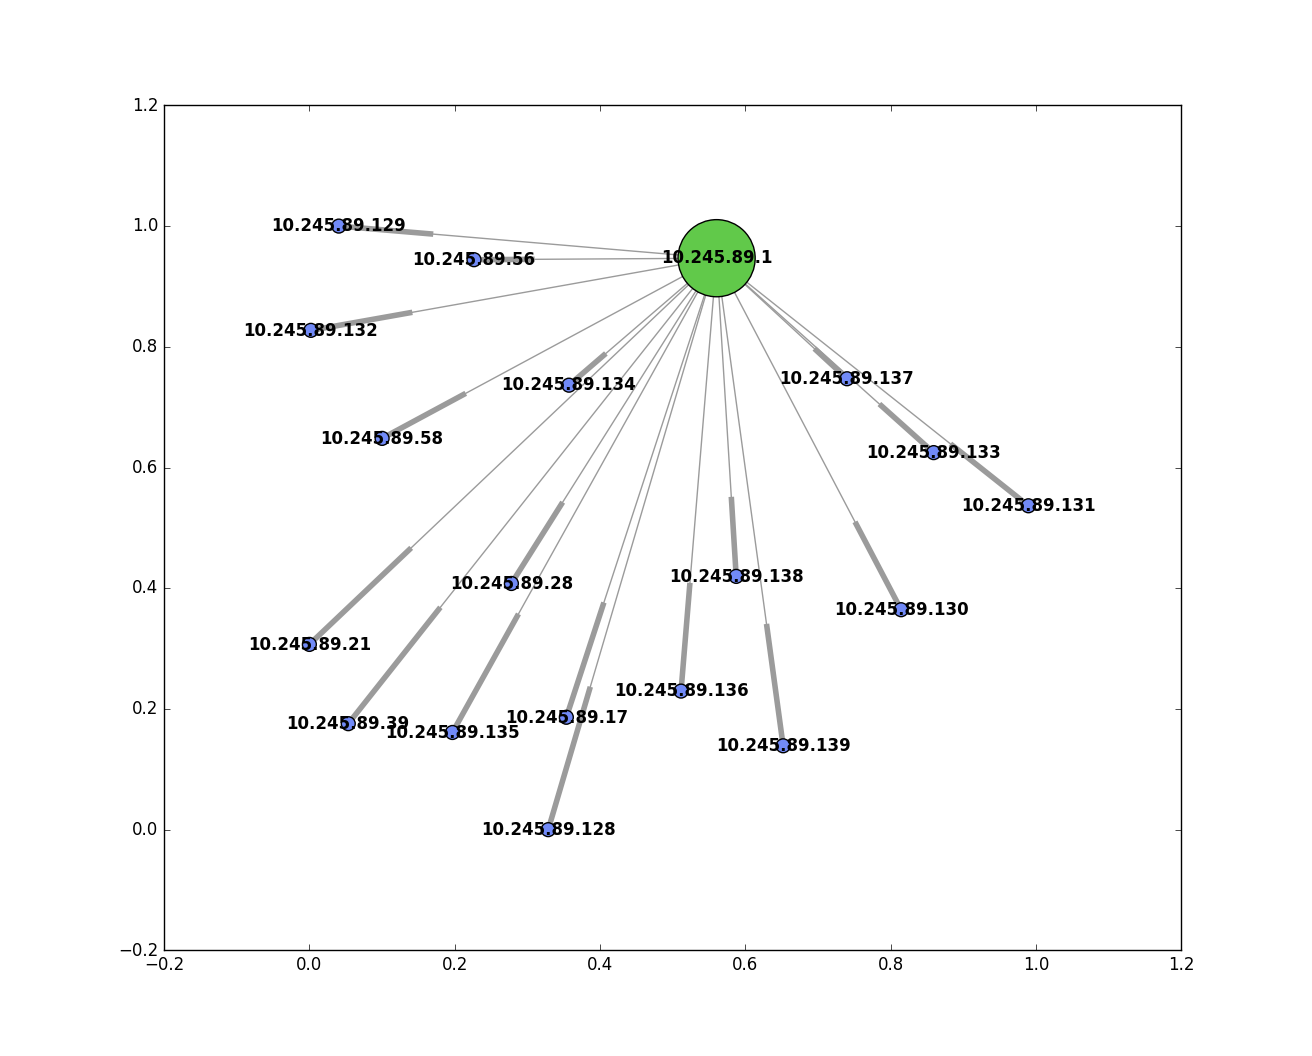
\includegraphics[scale=0.6]{imagenes/analisisTCORPcableada/cableada-12.png} 
\end{figure}

Quedaría, a futuro, realizar más experimentos en redes cableadas en orden de afirmar la hipótesis de que la fuente $S2$ funciona mejor para éstas.







